\documentclass[journal]{IEEEtran}
%\documentclass[12pt,journal,draftclsnofoot,onecolumn]{IEEEtran}
%\documentclass[conference]{IEEEtran}

\IEEEoverridecommandlockouts

\usepackage{etex}

%Fixing IEEEtran.cls bug with [english]{babel}
\makeatletter
\def\markboth#1#2{\def\leftmark{\@IEEEcompsoconly{\sffamily}\MakeUppercase{\protect#1}}%
\def\rightmark{\@IEEEcompsoconly{\sffamily}\MakeUppercase{\protect#2}}}
\makeatother

% \usepackage{t1enc}

\usepackage{listings}

%\usepackage[utf8x]{inputenc}
\usepackage[english]{babel}
\selectlanguage{english}
\usepackage{color}
\usepackage{lipsum}% http://ctan.org/pkg/lipsum
%\usepackage{caption}
\usepackage{cite}
\usepackage[pdftex]{graphicx}
%\usepackage{subfig}
%\usepackage{subcaption}
\usepackage{amsmath}
\usepackage{mathtools}
\usepackage{amsfonts}
\usepackage{array}
\usepackage{verbatim}
\usepackage{listings}
\usepackage{hyperref}
\usepackage{url}
\usepackage{enumerate}
\usepackage{multirow}

\usepackage{epsfig}
\usepackage{epstopdf}
\usepackage{multicol}% http://ctan.org/pkg/multicols
\usepackage[font=footnotesize]{caption}
\usepackage[font=scriptsize]{subcaption}
% Tikz
\usepackage{tikz}
\usepackage{pgfplots}
\pgfplotsset{compat=newest}
\pgfplotsset{plot coordinates/math parser=false}
\newlength\fheight
\newlength\fwidth
\usetikzlibrary{patterns,decorations.pathreplacing,backgrounds,calc}
\definecolor{SchoolColor}{RGB}{0.71, 0, 0.106}%181,0,27} unipd red
\definecolor{chaptergrey}{rgb}{0.61, 0, 0.09} % dialed back a little
\definecolor{midgrey}{rgb}{0.4, 0.4, 0.4}
\definecolor{chaptergreen}{rgb}{0.09, 0.612, 0}
\definecolor{chapterpurple}{rgb}{0.522, 0, 0.612}
\definecolor{chapterlightgreen}{rgb}{0, 0.612, 0.522}

%\raggedbottom

% Pseudocode
\usepackage[ruled, vlined]{algorithm2e}

\SetKwRepeat{Do}{do}{while}
\SetKwBlock{wpPa}{with probability $P_A$}{end}
\DontPrintSemicolon
% \usepackage{algorithm}
% \usepackage[noend]{algpseudocode}
% \renewcommand\algorithmicthen{}
% \renewcommand\algorithmicdo{}
\usepackage{lscape}

\addto\captionsenglish{\renewcommand{\figurename}{Fig.}}

\newcommand{\field}[1]{\mathbb{#1}}

\DeclareMathOperator*{\argmin}{arg\,min}
\DeclareMathOperator*{\argmax}{arg\,max}
\newcommand{\norm}[1]{\left\lVert#1\right\rVert}
\renewcommand{\arraystretch}{2}

\newcommand{\DP}[1]{\textbf{(DP: #1)}}
\newcommand{\el}[1]{\textr{(EL says: #1)}}
\newcommand{\fm}[1]{\texbf{(FM says: #1)}}

\usepackage{threeparttable}
%\usepackage[table,xcdraw]{xcolor}
\usepackage{tabularx}
\usepackage{multirow}
\usepackage{booktabs}
\newcommand{\tabitem}{~~\llap{\textbullet}~~}
\usepackage{array, blindtext}
\usepackage{wrapfig}
\usepackage{pdfpages}
\usepackage[acronym]{glossaries}

% use tikArchiviz images or eps
\newif\iftikz
\tikztrue

\graphicspath{{./figures/}}

\title{Heuristic optimization of Distributed Storage Network techniques}
\author{\IEEEauthorblockN{Federico Mason$^*$, Davide Peron$^*$, Enrico Lovisotto$^*$}\\
\small{{$^*$Department of Information Engineering, University of Padova -- Via Gradenigo, 6/b, 35131 Padova, Italy\\
Email: {\tt\{masonfed,perondav,lovisott\}@dei.unipd.it}\\}}
}

% Reduce the space below figs.
%\setlength{\belowcaptionskip}{-0.7cm}

%% Glossary
\newacronym{dsn}{DSN}{Distributed Storage Network}
\newacronym{edfc}{EDFC}{Exact Decentralized Fountain Codes}
\newacronym{adfc}{ADFC}{Approximate Decentralized Fountain Codes}
\newacronym{sa}{SA}{Simulated Annealing}
\newacronym{ga}{GA}{Genetic Algorithm}
\newacronym{jb}{JB}{Jumping Ball}
\newacronym{wsn}{WSN}{Wireless Sensor Network}
\newacronym{fp}{FP}{First Problem}
\newacronym{sp}{SP}{Second Problem}
\newacronym{of}{$f$}{Objective Function}
\newacronym{t}{T}{Temperature}
\newacronym{oc}{$x_o$}{Old Candidate}
\newacronym{nc}{$x_n$}{New Candidate}
\newacronym{sc}{$C_S$}{Step Coefficient}
\newacronym{ac}{$C_A$}{Acceptance Coefficient}
\newacronym{ap}{$P_A$}{Acceptance Probability}
\newacronym{ws}{$N_{WS}$}{Number of Worsening Steps}
\newacronym{wsmax}{$N_{WS}^{MAX}$}{ Maxiumum Number of Worsening Steps}
\newacronym{x}{x}{Candidate}
\newacronym{bestx}{$x_{best}$}{Best candidate}

\glsresetall
\begin{document}

\setlength{\belowcaptionskip}{-0.2cm}

% reduce space after title
\makeatletter
\patchcmd{\@maketitle}
  {\addvspace{0.5\baselineskip}\egroup}
  {\addvspace{-1.2\baselineskip}\egroup}
  {}
  {}
\makeatother

\maketitle

\begin{abstract}
In some previous works about \gls{dsn}, two packet spreading algorithm are presented, \gls{edfc} and \gls{adfc}.

Unfortunately the tuning of their fundamental parameters, $x_d$ and $\nu(d)$ respectively, was not thoroughly investigated.

We try to perform such tuning applying some heuristic optimization techniques, such as \emph{Simulated Annealing} and \emph{Genetic Algorithm}, in order to explore the solution space of the problem.

\end{abstract}

\begin{IEEEkeywords}
Distributed Storage Networks, sensors, heuristic optimization
\end{IEEEkeywords}

\glsresetall
\section{Introduction} \label{sec:introduction}
We consider a \gls{wsn} whose nodes are distributed over a known region.
Some of them, called \textit{sensing nodes}, collect and deploy data from the environment (temperature, pressure, motion data, \ldots) while the others, called \textit{caching nodes}, simply store data coming from \textit{sensing nodes}.

In literature, a \gls{wsn} often has a central node, a powered sink connected to the internet.
Such special node receives all information collected by the nodes in the network and provides it to the users.

However, in our paper, following what has been done in \cite{Lin2007}, we get rid of this assumption.
Users then must collect the data stored in the network visiting the geographical region where system is located.

In such a scenario, user visits only a certain number $h$ of nodes of the network.
Our reference paper \cite{Lin2007}, guarantees source packets decodability using \emph{Random Fountain Codes}, combining and spreading $K$ source packets across $N$ total nodes such that, using any group of $K+\epsilon$ of them (with $\epsilon$ constant in $K$), the original information can be successfully retrieved with high probability.

The challenge here is to keep the communication cost at a minimum level, while keeping the failure probability low.

Traditional but expensive two-way packet delivery is then discarded, in favour of one-way \emph{random walks}.
Random walks are designed according to \emph{Metropolis algorithm} such that the number of packets reaching each node resembles the Robust Soliton distribution, whose optimal decoding properties are known\cite{Luby}.

In this paper, we are going to find the optimal $x_d$ and $\nu(d)$ parameters for \gls{edfc} and \gls{adfc} respectively, with three different heuristics, and then test them with a network simulator, where further analysis is performed.

The article is structured in three sections.

In \autoref{sec:tech_approach} we present in detail the heuristic algorithms employed, first with a general description of the framework and then fucusing on our specific problem.

In \autoref{sec:results} we present the results obtained using the optimal parameter configurations in the network simulator we have implemented.

\section{Technical Approach}
\label{sec:tech_approach}

\gls{edfc} and \gls{adfc} spreading algorithms require their parameters $\vec{x}$ and $\nu$ to be tuned before executing them.

$\vec{x}$ is a K-dimensional variable of \gls{edfc} called \emph{redundancy coefficient}. Given a node with \emph{code degree} $d$, $x_d \cdot d$ represents the number of packets that should be received by the node itself at the end of packets spread.

The best value of $\vec{x}$ is the solution of the following optimization problem\cite{Lin2007}.

\begin{equation}
	\label{firstproblem}
	\begin{split}
		minimize & \quad \sum_{d=1}^K x_d d \mu (d) \\
		subject \ to & \quad \begin{dcases}
			Pr(Y<d|X=d) \leq \delta_d \\
			x_d \geq 1 \text{ ~for~ } d = 1,...,K
		\end{dcases}
	\end{split}
\end{equation}

$\nu$ is instead the degree distribution of network nodes such that, after package spread, the resulting degree distribution $\nu^\prime$ is as close as possible to the \emph{Robust Soliton Distribution}.

The optimal $\nu$ is the solution of the following optimization problem\cite{Lin2007}.

\begin{equation}
	\label{secondproblem}
	\begin{split}
		minimize & \quad \sum_{i=1}^{K/R}(\nu'(i)-\mu(i))^2 \\
		subject \ to & \quad \begin{cases}
			\sum_{i=1}^K \nu(i) = 1 \\
			\nu(i) \geq 0 \quad for \quad i=1,...,K
		\end{cases}
	\end{split}
\end{equation}

given
\begin{equation*}
	\begin{split}
		& v^\prime(i) = \sum_{d=1}^K \nu(d) \binom{K}{i} p(d)^i [1-p(d)]^{K-i} \\
		& p(d) = 1 - \left(1 -\frac{d}{N E}\right)^{\frac{N E}{K}} \\
		& E = \text{ expected value of }\nu
	\end{split}
\end{equation*}

From now on, we call \eqref{firstproblem} and \eqref{secondproblem} simply \gls{fp} and \gls{sp}.

We see immediately that \gls{fp} and \gls{sp} are not solvable with \emph{convex optimization} tecniques, as they don't minimize convex objective functions over convex sets.

To overcome this issue, we chose the heuristic approach, whose convergence to the optimum is not guaranteed in polynomial time, but whose effectiveness has been proven in many fields \cite{Edelkamp2010} where traditional tools (such as \emph{Simplex}) cannot be applied.

In fact the solutions obtained, despite not optimal, are still useful from a pragmatic point of view.

%TODO put here primitives of heuristic search? (now in SA chapter)

\subsection{Simulated Annealing}

The first algorithm we implement is known as \gls{sa}.
\gls{sa} is a probabilistic technique that takes ispiration from annealing in metallurgy, a process that aims to reduce materials defects.
In this physical process a piece of metal is warmed at high temperatures and then slowly cooled. In this way it is possible to achieve the molecular equilibrium inside the material itself.

In \gls{sa}, we treat \gls{of} as the internal energy of the material.
As in the physical process we want to reduce the function energy and slowly bring it to a stable value. In other words we want first to cross widely the function domain and then to concentrate in the points with higher probability to be the absolute minimum of \gls{of}.

\gls{sa} behaviour is dependent on a parameter called \gls{t}: relevant for the search are \gls{sc} and \gls{ac}, the number of points to inspect for given \gls{t} and the probability $P_A$ of accepting a point worse than the current, respectively.

At the beginning \gls{t} is initialized at a sufficient high value and then it is reduced at each algorithm step.

The process starts at a random point respecting problem constraints. Each new point $\vec{x}_{new}$ is found \emph{perturbing} previous vector $\vec{x}$ until a new valid one is found.

Empirically, we found for the two problems two different perturbation strategies, i.e. \emph{Neighbour} function in pseudocodes.
For \gls{fp} we add an uniform variable, whose range is proportional to temperature, to a randomly chosen component of the $\vec{x}$ vector, while for \gls{sp} we perturb ``moving'' some probability from one degree to one other, chosen uniformly across the distribution.

Such solution is kept or rejected according to the \gls{ap}, whose expression is the following.

\begin{equation*} \label{accept_prob}
	\begin{split}
	P_A(T) &= \begin{cases}
		1 & \Delta < 0 \\
		\exp{ \left( - C_A ~ \Delta / T \right) }
		& \Delta \geq 0
	\end{cases} \\
	\text{where } \Delta &= f(\vec{x}_{new})-f (\vec{x})
	\end{split}
\end{equation*}


The best point among all the explored ones is kept across the path and it is returned at the end of the computation.

The algorithm is provided here as pseudocode in \autoref{algo:SA}.

\begin{algorithm}
\KwIn{Objective function $f$ and constraints, Initial Temperature,  Maximum number of steps, Steps Coefficient, Acceptance Coefficient}
\KwOut{Optimal solution}
\caption{Simulated Annealing} \label{algo:SA}

$T \gets$ Initial Temperature \\
$x \gets$ Random valid point() \\
$x_{best} \gets x$ \\
$C_A \gets$ Acceptance coefficient \\
$N_S \gets 0$ \\
$N_S^{MAX} \gets $ Maximum number of steps \\

\While{$N_S < N_S^{MAX}$} {
	$C_S \gets$ Steps coefficient ($T$) \\
	\For{$i = 1$ to $C_S$} {
		$\vec{x}_{new} \gets$ Neighbour$(\vec{x})$\\
		$P_A \gets$ Acceptance probability($\vec{x}$, $\vec{x}_{new}$, $C_A$) \\
		\wpPa {
			$\vec{x} \gets \vec{x}_{new}$\\
		}
		\If{$f(x)<f(x_{best})$}{
			$x_{best} \gets x$\\
		}
		Increment $N_S$
	}
	update $T$\\
	update $C_S$\\
}
\Return{$x_{best}$}
\end{algorithm}

\subsection{Jumping Ball}

Our second search algorithm is a variation of \gls{sa}, called \gls{jb}, designed and implemented by our group.

Its approach rose from the observation that if the cooling phase of \gls{sa} takes to a sub-optimal region of the solution space there is no way to leave it for a better one.

So, we develop the heuristic of \emph{jumps}, whose aim is to overcome this issue. If the best solution available is not improved for a certain number $N_{WS}^{MAX}$ of small steps, as done in \gls{sa}, a \emph{jump} is performed perturbating lots of components all at once of a big extent.

$N_{WS}^{MAX}$ has to be initialized properly: a value too low would lead the algorithm to jump indefinitely without ever stabilizing in a single area, but a value too high would make jumps impossible, making pointless this variation.

A proper value instead enhances the exploration space of the \gls{sa} algorithm, leading to hopefully better results in our variant \gls{jb}.

The pseudocode for \gls{jb} is the same as \gls{sa}, the different \emph{Neighbour} function is described in \autoref{algo:JB_neigh}.

\begin{algorithm}
	\caption{Jumping Ball \emph{Neighbour}}\label{algo:JB_neigh}
	\KwIn{Problem constraints and objective function $f$, $\vec{x}$, $N_{WS}^{MAX}$, current number of worsening steps $N_{WS}$}
	\KwOut{$\vec{x}_{new}$}
	\Repeat{$\vec{x}_{new}$ respects constraints} {
		$\vec{x}_{new} \gets \vec{x}$ \\
		\If { $N_{WS} > N_{WS}^{MAX}$ } {
			\Repeat{$\vec{x}_{new}$ respects constraints} {
				Perturb an random number of components of $\vec{x}_{new}$
			}
			$N_{WS}$ = 0
		}
		\Else {
			Perturb just one component of $\vec{x}_{new}$ in $[1, K]$
		}
	}
	\If { $f(\vec{x}_{new}) > f(\vec{x}_{best})$  } {
		Increment $N_{WS}$
	}
	\Return $\vec{x}_{new}$
\end{algorithm}

\subsection{Genetic Algorithm}

Our third technique is an implementation of \gls{ga}, framework that takes randomly an initial set of solutions for the problem and tries to evolve this \emph{population} of points toward better values.

According to the biological interpretation, each candidate solution, in our case a multi-dimensional vector, is an \emph{individual}.
Then each of its components is called \emph{chromosome} or \emph{genotype} and the subsequent iterations to explore the solution space \emph{generations}.

In each step of the algorithm the worst performing individuals of the current population are discarded and replaced by \emph{mutations} of the best individuals, which survives to the next round.

In this work we have decided to keep the 25\% best individuals of the current generation for the next one and obtain the remaining three quarters perturbing one, two and three components of the previous ones respectively.

Perturbations are performed as described earlier in \gls{sa} section.

\begin{algorithm}
	\KwIn{Objective function and constraints, survival rate, max generations, population size}
	\KwOut{Optimal solution}
	generation $\gets 0$\\
	best part size $\gets$ population size $\cdot$ survival rate\\
	population $\gets$ get initial population\\
	\While{\emph{generation} $<$ \emph{max generations}}{
		sort(population)\\
		\For{$j=1$ to \emph{round(1/survival rate)}}{
			\For{$i=1$ to \emph{best part size}} {
				population(j $\cdot$ best part size + i) $\gets$ population(i)\\
				\Repeat{\emph{individual} respect constraints}{
					individual $\gets$ population(j $\cdot$ best part size + i)\\
					candidates(0) $\gets$ individual + perturbation\\
					candidates(1) $\gets$ candidate(0) + perturbation\\
					candidates(2) $\gets$ candidate(1) + perturbation\\
					sort(candidates)\\
					individual $\gets$ candidates(0)
				}
				population(j $\cdot$ best part size + i) \\
			}
		}
		generation++ \\
	}
	\Return{population(0)}
	\caption{Genetic Algorithm}\label{algo:GA}
\end{algorithm}

Our \gls{ga} can be tuned with the following parameters.
\begin{description}
	\item[\textbf{Survival Rate}] \hfill \\
	The fraction of population that is used to create the next generation. A survival rate too high forces the algorihm to discard worse, but potentially interesting paths in favour of the current best, while a value too low reduces the progress across generations.
	\item[\textbf{Max Generations}] \hfill \\
	Number of generations, the iterations of the algorithm. Note that exploration time is linear in this parameter.
	\item[\textbf{Population size}] \hfill \\
	Number of individual in a population. Increasing this parameter enhances performances but increase slightly the memory load and to a greater extent computation time.
\end{description}

\section{Results}
\label{sec:results}
\begin{figure}
  \centering
	    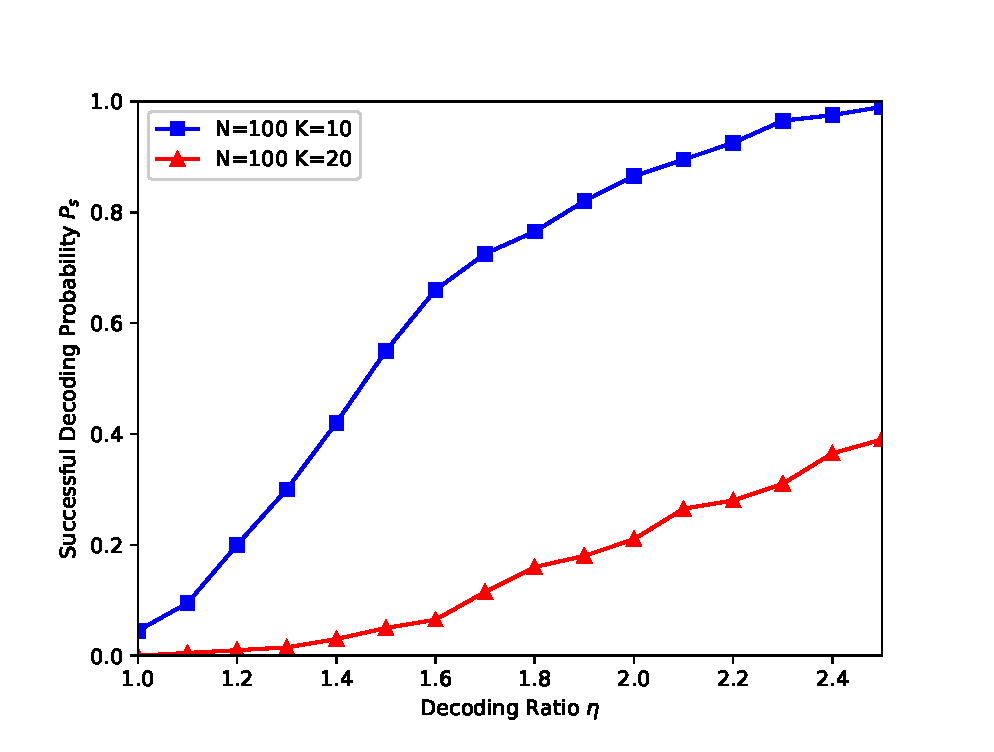
\includegraphics[width=0.9\columnwidth]{ratiovsprob.eps}
  \caption{Successfull decoding probability $P_s$ for different values of $N$, $K$ and decoding ratio $\nu$.}
  \label{fig:ratiovsprob}
\end{figure}

\section{Conclusions And Future Work}
\label{sec:conclusions}

\bibliographystyle{IEEEtran}
\bibliography{bibliography}

\end{document}
